\label{chapter:sheriff}

We provide two tools, \SheriffDetect{} and \SheriffProtect{}, to attack
the false sharing problems of multithreaded programs. 
These tools are based on the same \sheriff{} framework.

\section{\sheriff{} framework}
\label{sec:framework}

\Sheriff{} is a drop-in replacement of \pthreads{} library, which is a standard threading 
library in Linux system: there is no need to change the 
existing operating system, to change the source code or to recompile the code, 
we can link to \Sheriff{} library directly or dynamicallyy 
linking to \sheriff{} framework using LD\_PRELOAD mechanism. 

% Benefit of "processes-as-threads} concept.
\Sheriff{} extends the \emph{processes-as-threads} concept introduced
in our Grace~\cite{grace} work.
\Sheriff{} intercepts those threads spawning calls:
instead of spawning new threads, \sheriff{} calls \texttt{clone} to 
fork processes with the shared file descriptor table but with different address spaces.
Because different processes have different address spaces, 
\sheriff{} can isolate executions from different threads, 
providing the ``per-thread-isolation'' functionality.
Since each process has its own separate page table entries, we can set up different 
protection permissions for the same pages inside different processes, 
providing the ``per-thread-protection'' mechanism.

% The basic machnism of sheriff? How to utilize the per process isolation and protection.
\sheriff{} maintains two file-backuped mappings for both the globals and the heap: 
a per-process private mapping for applications to work on directly, 
and a shared mapping to hold the shared state across different processes.
The private mapping is connected to the shared mapping by mapping to the same file.
\sheriff{} works as follows: 
reads initially access the shared mapping directly;
\sheriff{} creates a per-process private page after the first write on a page; 
%invoking a copy-on-write operation in the underlying operating system, 
both reads and writes only access this local private page afterwards. 
Normally applications can only update the private mappings, it is the duty of 
\sheriff{} runtime system to maintain the shared memory semantics:
\sheriff{} merges those per-process modifications to the shared mapping and releases those 
temporary private pages at synchronization boundaries. 

\subsection{Twinning-and-diffing mechanism}
\label{sec:twinning-and-diffing}
In order to find out those per-process modifications, 
\sheriff{} relies on  the twinning-and-diffing mechanism, 
adapted from existing distributed shared memory systems, such as 
TreadMarks and Munin~\cite{dsm:munin, dsm:treadmarks}.

\sheriff{} relies on ``per-thread-protection'' mechanism to provide the twinning-and-diffing mechanism: 
\sheriff{} write-protects all pages of private mappings initially so that it
can discover write operations by handling page faults of access violation;
In the page fault handler, \sheriff{} creates a twin page for each faulted page (\textbf{twinning}), 
which keeps the initial state of a page;
%A twin page keeping the initial state of a page, is created in the access violations handler.
\sheriff{} also creates a working page utilizing the copy-on-write mechanism of underlying 
operating system, which always has the final state of a written page. 
By simply comparing the difference of the working page against its corresponding twin page 
(\textbf{diffing}), 
\sheriff{} can determine actual modifications of a process.
 
It is essential that a twin page should be identical to its working page initially, 
otherwise we can not find those actual modifications exactly. 
\sheriff{} forces a copy-on-write operation on a specific address explicitly in the page fault handler:
it reads the value from the head of this page and writes this value back. 
By creating a twin page from this private working page, \sheriff{} can guarantee the identicalness between the twin page and its working page.
 
\subsection{Executions of \sheriff{}}
\label{sec:sheriff-execution}

\begin{figure}[!t] 
\centering
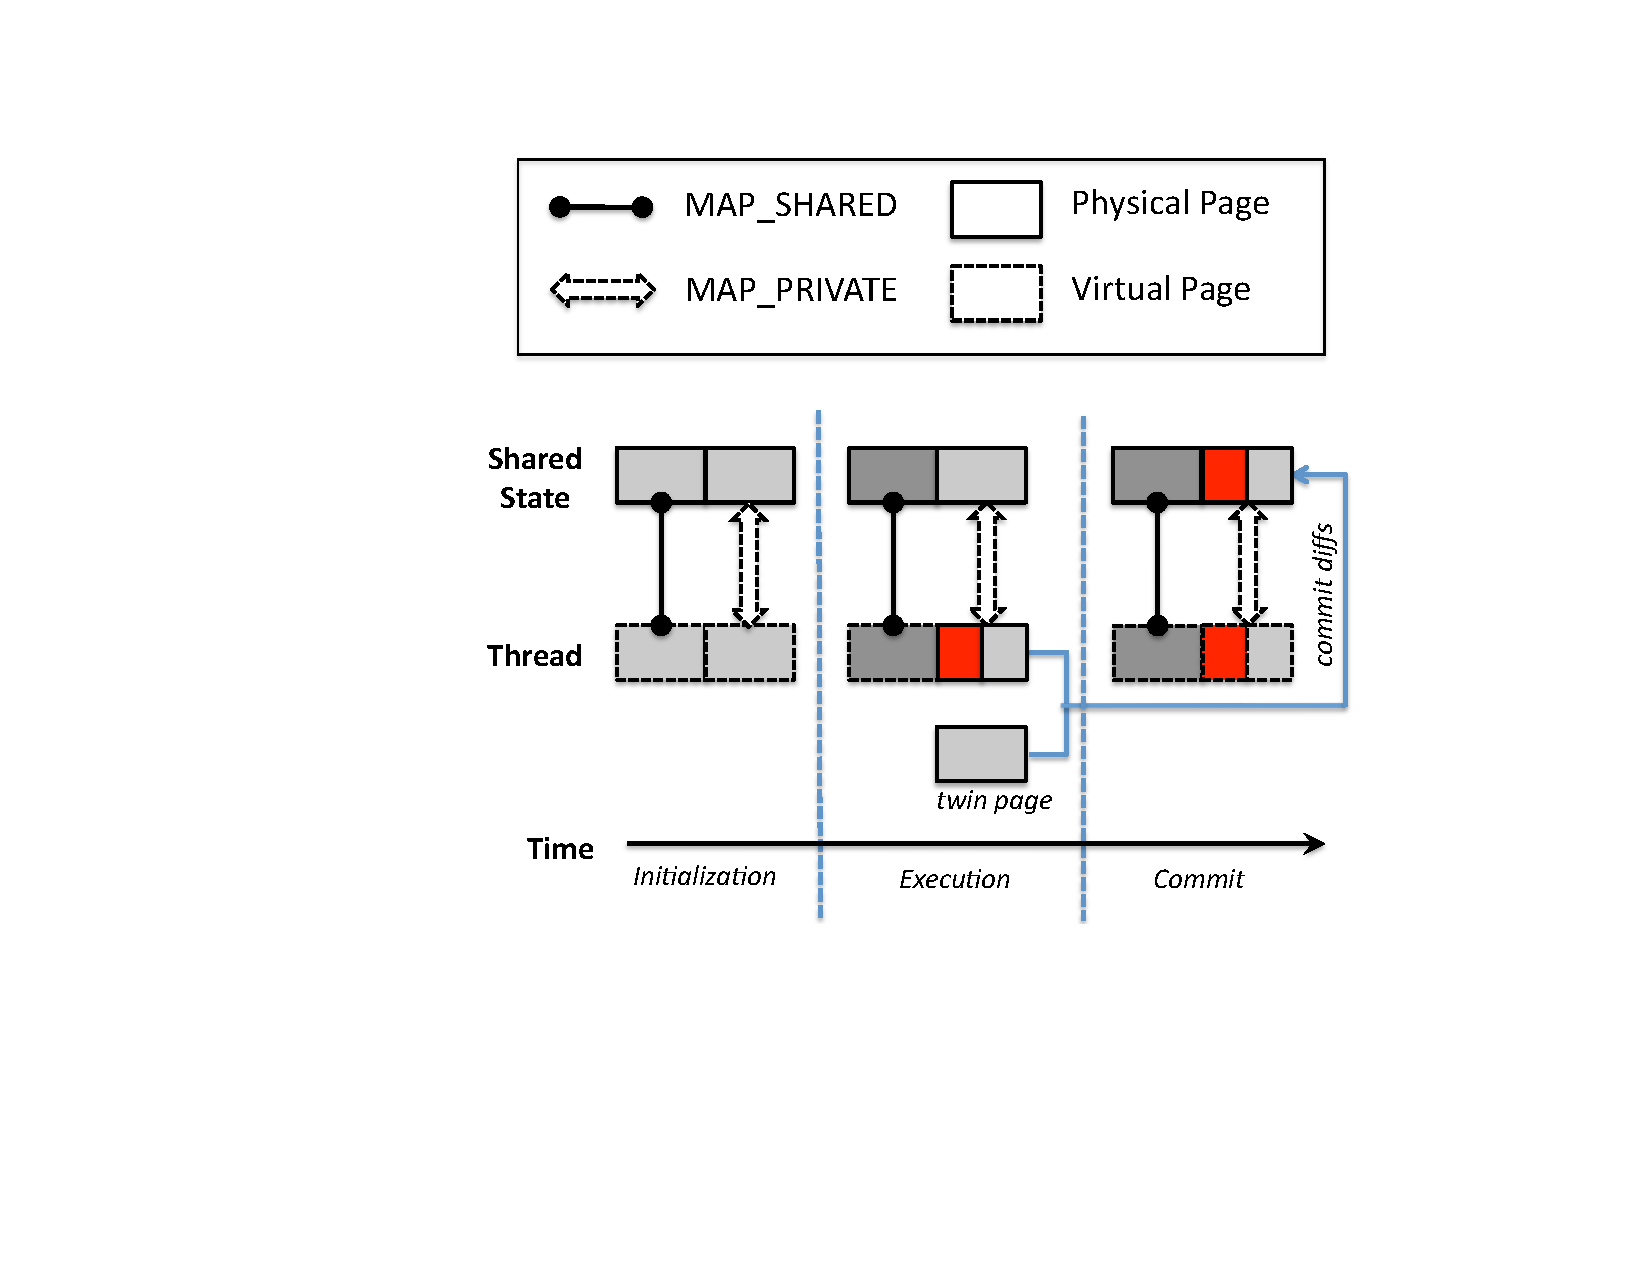
\includegraphics[width=3.5in]{sheriff/figure/sheriffframework.pdf}
\caption{\sheriff{} execution inside a transaction
\label{fig:sheriffoverview}}
\end{figure} 

\sheriff{} intercepts all threads synchronizations and breaks the whole execution of each thread to 
multiple transactions based on synchronization boundaries: 
those sections of each thread between synchronization points and critical sections
are considered as separate transactions.
Those synchronizations includes locks, conditional variables, barriers and 
various types of thread exits and signals.
\sheriff{} wraps all synchronizations in a similar way as the following example:
a call to \texttt{pthread\_mutex\_lock} first ends the current transaction; 
\sheriff{} calls \pthreads{}'s process-shared \texttt{pthread\_mutex\_lock};  
\sheriff{} starts a new transaction after the lock is acquired and ends at the next 
possible synchronization operation, one of \texttt{pthread\_mutex\_unlock}, 
\texttt{pthread\_cond\_wait} or \texttt{pthread\_cond\_signal} calls.
Figure~\ref{fig:sheriffoverview} shows the execution in a single transaction. 

\textbf{Transaction Begin:}
In the beginning of every transaction, \sheriff{} write-protects all private pages in order to
capture writes on those pages by handling \texttt{SEGV} protection faults.  

\textbf{Execution:} In the execution phase, reads on non-faulted pages in this transaction 
are performed on the shared mapping directly. The first write on
a protected page invokes a page fault. By handling this fault,  
\sheriff{} records those faulted pages, creates twin pages 
and unprotects them so that future accesses can run at full speed.  

\textbf{Transaction End:} At the end of each transaction, \sheriff{} 
commits local changes of each process to the shared mapping by using twinning-and-diffing mechanism, 
reclaims those temporary pages and
recovers the permissions for those pages written in this transaction. 
   
Through this, \sheriff{} achieves the same semantics as 
that of \pthreads{} for programs without races
and \texttt{ad hoc} synchronizations (see~\cite{ad-hoc-considered-harmful} for the definition).
% shared variables accesses should be synchronized correctly.

%\subsection{Difference with \grace{}}
%\sheriff{} extends the processes-as-threads concept introduced by \grace{} but
%with different semantics, generality and goals. 

%\grace{} is designed to tolerate concurrency errors by imposing a sequential semantics. 
%\grace{} only supports fork-join programs without inter-thread communications (e.g. conditional 
%variables and barriers), relying on a rollback mechnism to ensure  
%sequential semantics and determinism. 

%\sheriff{} supports general multithreaded programs without any annotations or changes of
%programs. \sheriff{} does not prevent the usage of inter-thread synchronizations at all. 
%Since there is no rollback mechanism and protections on read operations, 
%\sheriff{} generally runs much
%faster than \grace{}, without any guarantee of determinism.

\section{False Sharing Detection}
% How to find out the "false sharing problem" ? We are trying to get those callsite information. 
% False sharing problem means that two threads are accessing different words in the same cache line
% and one of them is a read operations. 
\SheriffDetect{} is a tool to detect false sharings of multithreaded programs, built on
top of the \sheriff{} framework. 
As we described in Section~\ref{falsesharing}, false sharing can greately slow down the program 
when there are a lot of interleaved writes from different threads on the same cache line.
\SheriffDetect{} captures all cache lines with interleaved writes and 
ranks the seriousness by the frequency 
of interleaved writes: cache lines with more interleaved writes are considered to have more 
performance impact on the programs.  

Relying on ``per-thread-isolation'' and ``per-thread-protection'' mechanisms to track written pages, 
combining with twinning-and-diffing mechanism (explained in Section \ref{sec:twinning-and-diffing}),
\SheriffDetect{} can find out per-process modifications in the end of each transaction.
However, for a long transaction, checking in the end of each transaction is not enough because it
may loose multiple modifications inside each transaction.
So \SheriffDetect{} periodically samples the modifications for those long transactions. 

Based on this, \SheriffDetect{} utilizes the following mechanisms to report false 
sharings precisely and accurately. 

\begin{itemize}

\item  
In order to precisely report origins of false sharing objects, \SheriffDetect{} keeps callsite 
information for each heap object and reports the source code level information about 
each object. 

\item
%In order to avoid reporting true sharing problems, 
\SheriffDetect{} tracks modifiers and numbers of modifications for each word so that 
\SheriffDetect{} can only reports a cache line with actual false sharing problems.  
In the meanwhile, numbers of modifications on each word helps to identify 
actual causes since there are multiple fields or multiple objects 
in the same cache line.  

\item
To avoid the pseudo false sharing problems caused by memory re-usages, 
\SheriffDetect{} intercepts the memory allocations and deallocations functions 
and handles them correspondingly. \SheriffDetect{} is the first work to observe and deal 
with problems caused by memory re-usage.
%When an objectXXXXXXXXXXX 

\end{itemize}  

In conclusion, \SheriffDetect{} is the first practical tool, 
only introducing 21\% performance overhead,to locate false sharing
problems precisely and accurately.
Now the tool is used by \texttt{SAS} and \texttt{Intel} company 
to detect false sharings of their actual products. 
However, it is impossible for \SheriffDetect{}
to identify read operations with reasonable overhead,  
so \SheriffDetect{} can not be used to detect read-write false 
sharing problems: one writer and multiple 
readers in the same cache line.

% Problem of this approach, we can't detect the single-writer cases. 

\section{False Sharing Prevention}
% What is the basic idea of \sheriffProtect{}.

We observes a fact from \SheriffDetect{}: isolating executions of 
different threads actually improves performance for those programs with serious false sharings.
Here, different processes actually access different physical pages after the first 
write inside a transaction, the ping-pong effect of loading-and-invalidating is actually prevented by doing this. 

Based on this observation, we developed \SheriffProtect{} to tolerate false sharings
of multithreaded programs utilizing the following mechanisms. 

\begin{itemize}
\item
\SheriffProtect{} only makes pages private when it is beneficial to do this. 
A private page can tolerate false sharings while introducing 
different types of overhead inside a transaction: 
protection overhead in the beginning, 
page fault and commit overhead for those written pages and the overhead to reclaim temporary pages 
in the end.
When a page does not have false sharings, 
the overhead can slow down the execution and should be avoided as much as possible.
In out implementation, \SheriffProtect{} only prevents the false sharings
on small objects (those less than 1024 bytes in size) and all large objects 
are mapped shared without any protection. 
 

\item
Short transactions does not give any performance benefit because the overhead we mentioned above
can be larger than the benefit by preventing false sharings.
\SheriffProtect{} employs a simple adaptive mechanism to avoid this problem: 
we only protect the memory when a transaction is longer than a specific threshold. 
However, this approach also means that we can not tolerate false sharings for 
programs with intensive synchronizations. 
For a program with intensive synchronizations, 
it is better to rely on
\SheriffDetect{} to find false sharings and fix it manually.  

\end{itemize}
 

% What is the result of \sheriff{}.
